\section{Expérimentation}\label{sec:experimentation}
% les differentes experimentations faites pour comparer les differents chases
% commentaires pour chacun

Dans cette section nous présentons une évaluation exhaustive des différents chases. Nous avons trois objectifs principales en réalisant cette évaluation :

\begin{enumerate}
  \item Vérifier l'exactitude des nos chases.
  \item Comparer nos chases à ceux qui existaient déjà dans Graal.
  \item Comparer tous les différents chases implémentés. 
\end{enumerate}

\subsection{Méthode d'expérimentation}

Nous avons implémenté un outil de benchmarking qui nous permets de lancer tous les chases (ceux qui nous avons implémenté aussi que ceux déjà existants dans Graal) avec des limites sur les temps global d'exécution, le temps d'exécution de chaque étape de largeur et le nombre des faits générés. Étant donné que les chases peuvent facilement exploser en termes de temps d'exécution et faits générés on a implémenté ces limites pour éviter des temps d'exécution trop longs et des possibles erreurs de mémoire. 

Le benchmark prends en entrée un fichier "dlp" avec la base des connaissances et procède à la saturer itérativement avec chacun des chases jusqu'à ce que la saturation soit fini ou l'une des trois conditions d'arrêt mentionnés précédemment soit atteint. Une fois la saturation est fini on sauvegarde comme résultat le temps d'exécution de chaque étape et le nombre de faits qui contient la base de faits à la fin de chaque étape ce qui nous permets de faire des comparaisons détaillés entre tous les chases executés.

Cette méthode d'expérimentations nous a permis d'accomplir les objectifs définis au début de cette section. Le nombre de faits générés nous permets de vérifier l'exactitude de nos chases par rapport au chases existants en graal, une fois les chases ont été validés le temps d'exécution nous permets de comparer l'efficacité de nos chases par rapport aux chases existants. Et finalement avec ces deux mesures nous pouvons aussi comparer tous les chases en terme de vitesse d'exécution et de capacité à éviter les redondances.

\subsection{Base de connaissances d'expérimentation}

Nous avons pris plusieurs base des connaissances pour tester les chases, d'abord nous avons pris des petites base de connaissances faites pour nous qui ont la particularité d'avoir peu de règles et peu des faits au départ mais qui génèrent des nombreuses redondances ce qui pousse les algorithmes après peu d'itérations, ensuite, nous avons aussi testé avec des gros bases de connaissances crées par la communauté scientifique qui ont été crées explicitement pour pousser les algorithmes de chase aux limites. Nos bases des connaissances sont les suivants : 

\vspace{10pt}
\textbf{ex0.dlp}\\
$\mathcal{F} = \{p(a,b)\}$ \\
$R = p(X,Y) \rightarrow p(Y,Z), p(Z,Z), p(Z,X), p(X,U), p(U,Y), p(U,U)$\\

\textbf{ex1.dlp}\\
$\mathcal{F} = \{p(a,b)\}$ \\
$R = p(X,Y) \rightarrow p(Y,Z), p(Z,U), p(U,X), p(X,O), p(O,Q), p(Q,Y), p(U,U), p(Q,Q), p(O,O), p(Z,Z)$\\

\textbf{ex11.dlp}\\
$\mathcal{F} = \{p1(a), p1(n),q(b,f),q(f,c),q(b7,f5),q(f5,c5),q(b6,f6),q(f8,c8)\}$ \\
$R = p1(X), q(V,Y) \rightarrow p1(Z),p(X,Z),q(V,Z)$\\

\textbf{ex2.dlp}\\
$\mathcal{F} = \{p(c,d), p(a,b), p(e,f)\}$ \\
$R = p(X,Y), p(U,W) \rightarrow q(X,Z), q(Z,X), p(Z,V), q(U,Z), q(Z,U)$\\

\textbf{example.dlp}\\
$\mathcal{F} = \{b(a), c(a)\}$\\
$R1 = b(X) \rightarrow p(X,Z)$\\
$R2 = p(X,Y) \rightarrow p(X,Z), a(Z)$\\
$R3 = p(X,Y), a(W) \rightarrow p(Y,Z)$\\
$R4 = p(X,Y), a(Y) \rightarrow p(Y,Y)$\\
$R5 = p(X,Y), c(X) \rightarrow q(Y)$

\subsection{Résultats}

Tous les expérimentations ont été réalisés dans un seul ordinateur avec les spécifications suivantes : (Processeur, mémoire, etc). Les paramètres d'arrêt utilisés lors du benchmark sont 1 heure de temps de exécution, 30 minutes maximum par étape et 1.000.000 de faits générés.

\subsubsection{Comparaison Graal Chases et Nouveaux Chases}

Nous commençons d'abord pour comparer les temps d'exécution du Semi-Oblivious Chase et Restricted Chase qui sont implémentes dans Graal avec nos nouvelles versions. L'axe Y a été mis en échelle avec une fonction logarithme pour que les graphiques restent lisibles.

\begin{figure}[H]
\centering
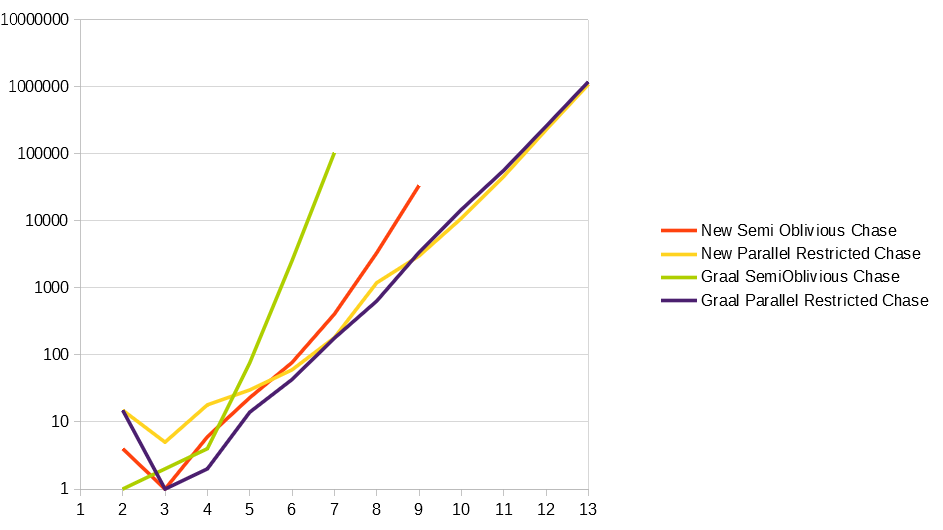
\includegraphics[width=\textwidth]{pictures/benchmark old-new/ex0oldnew.png}
\caption{ex0}
\label{fig:ex0oldnew}
\end{figure}

\begin{figure}
\centering
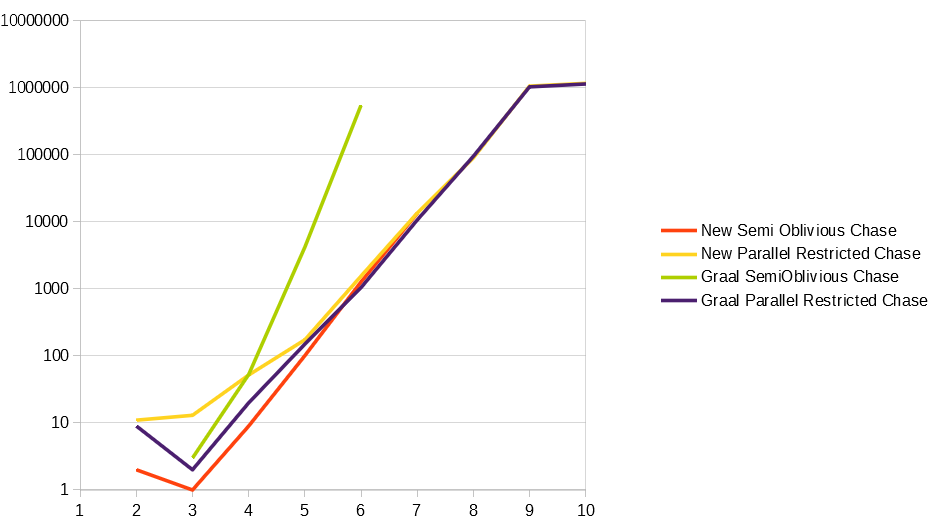
\includegraphics[width=\textwidth]{pictures/benchmark old-new/ex1oldnew.png}
\caption{ex1}
\label{fig:ex1oldnew}
\end{figure}

\begin{figure}
\centering
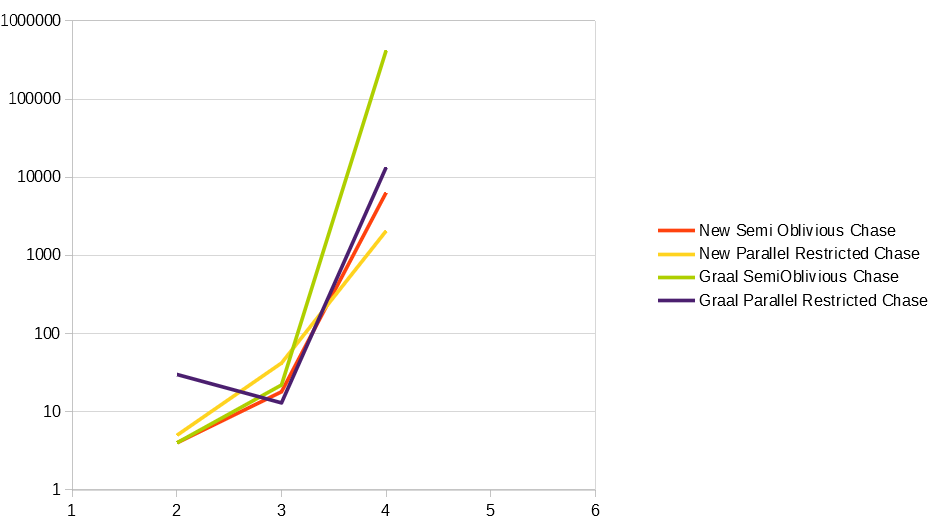
\includegraphics[width=\textwidth]{pictures/benchmark old-new/ex2oldnew.png}
\caption{ex2}
\label{fig:ex2oldnew}
\end{figure}

\begin{figure}
\centering
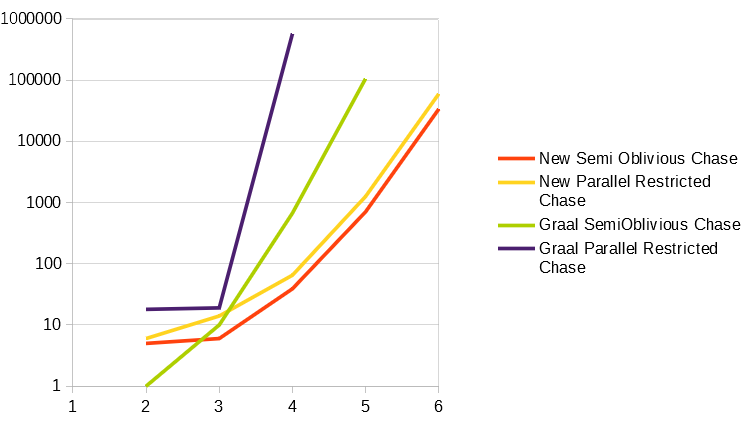
\includegraphics[width=\textwidth]{pictures/benchmark old-new/ex11oldnew.png}
\caption{ex11}
\label{fig:ex11oldnew}
\end{figure}

\begin{figure}
\centering
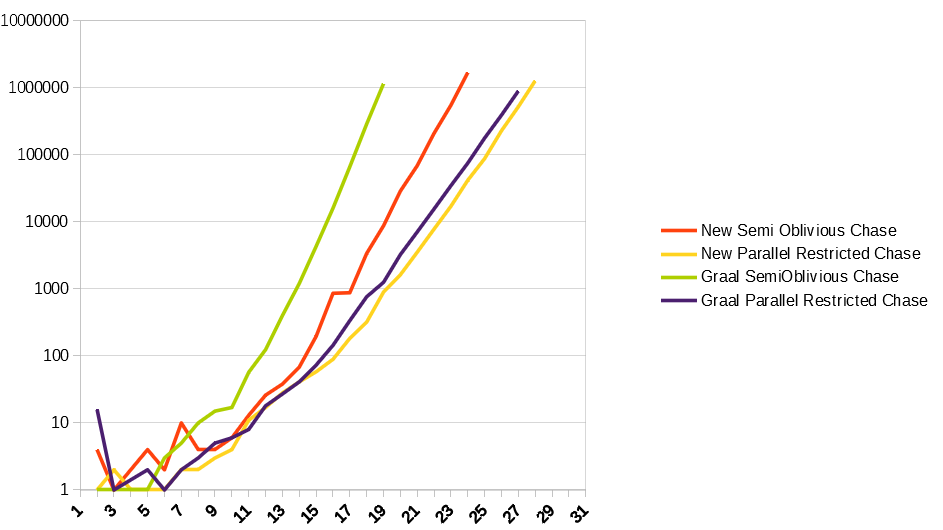
\includegraphics[width=\textwidth]{pictures/benchmark old-new/exampleoldnew.png}
\caption{example}
\label{fig:exampleoldnew}
\end{figure}

Nous pouvons constater que dans la plupart des cas  nos chases sont plus rapides que les versions déjà implémentés dans Graal, on remarque qu'au début quand la base de faits est petite les Graal Chases sont légèrement plus rapides, néanmoins, une fois que la base de faits commence à grandir les nouveaux chases deviennent considérablement plus rapides, cela est du principalement à notre méthode des calcul des nouveaux homomorphismes qui au début ajout du calcul additionnel mais quand la base commence à grandir elle nous évite de recalculer des nombreaux homomorphismes redondants.

\subsubsection{Comparaison Nouveaux Chases}

Ici, nous nous intéressons à comparer les nouvelles versions du restricted chase, le core chase, le local core chase et le vacuum chase.

La base de connaissances Example.dlp donne donne des résultats très intéresants (Fig. \ref{fig:examplenewfacts} et  Fig. \ref{fig:examplenewtime}), l'algorithme qui prend le plus de temps c'est le Parallel Restricted Chase, cela est du au fait qu'il genere des nombreux faits redondants, après nous avons le vacuum chase qui est capable d'éliminer un grand nombre des faits redondants ce qui le rends plus efficace que le Parallel Restricted Chase en temps d'execution aussi qu'en quantité des faits génerés. Ensuite nous avons le Local Core Chase et le Breadth First Restricted Chase qui sont equivalents en termes de faits produits, cela peut s'expliquer car le Breadth First Chase a réussi a trouver un ordre d'application des règles qui est equivalent au Local Core Chase, et comme attendu le Breadth First Chase est beacoup plus rapide que le Local Core Chase car il fait moins des calculs. Finalement nous avons le Core Chase qu'ici fini en 5 étapes avec une base de faits contenant 6 faits ce qui le rends l'algorithme le plus efficace en nombre de faits de produits, et aussi en temps car la saturation est fini.

\begin{figure}
\centering
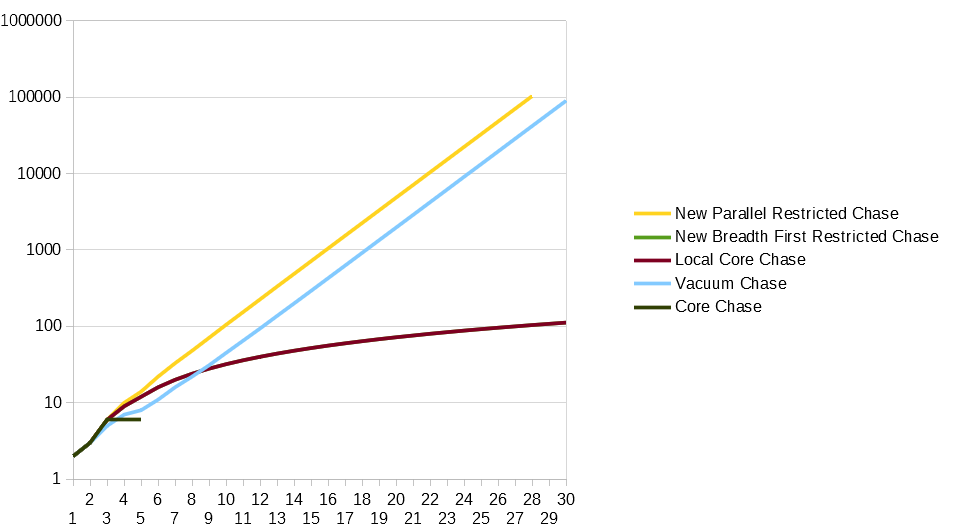
\includegraphics[width=\textwidth]{pictures/benchmark new/examplenewfacts.png}
\caption{example.dlp Faits générés}
\label{fig:examplenewfacts}
\end{figure}

\begin{figure}
\centering
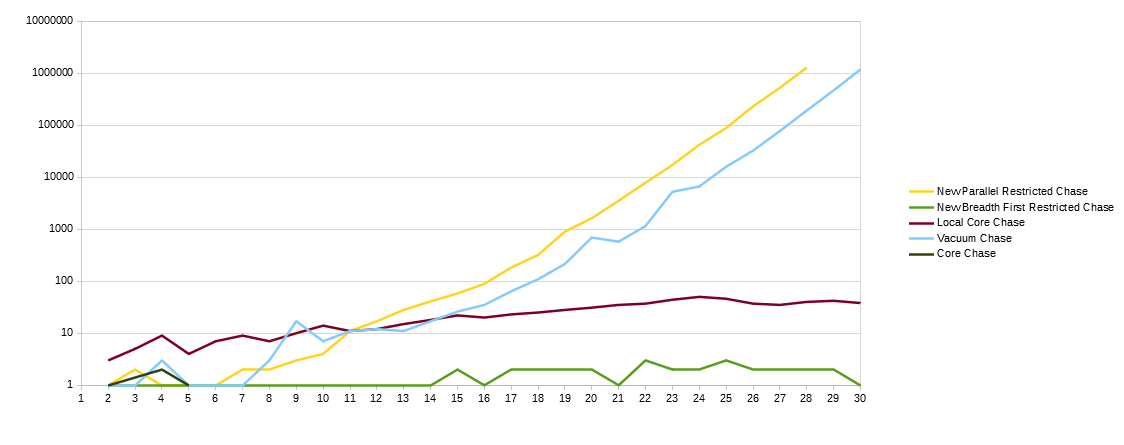
\includegraphics[width=\textwidth]{pictures/benchmark new/examplenewtimes.png}
\caption{example.dlp Temps}
\label{fig:examplenewtime}
\end{figure}